\chapter{Organisation et gestion de données}
{https://sacado.xyz/qcm/parcours_show_course/0/117141}
{
\begin{CpsCol}
 \textbf{Les savoir-faire du parcours}
 \begin{itemize}
 \item Savoir lire des données dans un tableau.
 \item Savoir compléter un tableau.
 \item Savoir utiliser un diagramme en bâtons.
 \item Savoir construire un diagramme en bâtons.
 \item Savoir utiliser un diagramme circulaire.
 \item Savoir construire un diagramme circulaire.
 \item Savoir utiliser un diagramme cartésien.
 \item Savoir construire un diagramme cartésien.
 \end{itemize}
\end{CpsCol}
}

\begin{pageCours} 

\section{Tableaux}

\begin{DefT}{Tableau simple}
Les \textbf{tableaux} permettent d'organiser et de regrouper des données pour les lire plus facilement.
\begin{itemize}
\item On utilise un tableau à \textbf{une seule entrée}\index{Simple|Tableau} pour organiser des données selon \textbf{un seul critère}.
\item On utilise un tableau à \textbf{double entrée}\index{A double entrée|Tableau} pour organiser des données selon \textbf{deux critères}, l'un qui est lu en ligne et l'autre en colonne.
\end{itemize}
\end{DefT}


\begin{Ex}{Tableau simple}

On a mesuré la taille d'une pousse de bambou  lors des 6 premiers mois après sa plantation.
 \begin{center}
 \begin{tabular}{|c|c|c|c|c|c|c|} 
  \hline
  Mois & Novembre & Décembre & Janvier  & Février & Mars & Avril \\
  \hline
  Taille (cm) & $70$ & $100$ & $127$ & $150$ & $180$ & $212$  \\
  \hline
 \end{tabular}
 \end{center}

La pousse de bambou mesurent $70$ cm lors de sa plantation. Au mois de février, elle mesure $150$ cm.
\end{Ex}


\begin{Ex}{Tableau à double entrée}
Voici les résultats d'une enquête réalisée dans un collège sur le moyen de locomotion des élèves.
 \begin{center}
 \begin{tabular}{|c|c|c|c|c|c|c|}
  & A pied & Voiture & Bus &  Vélo & Autres & Total \\  \hline
  Garçons & $92$ & $36$ & $118$ & $54$ & $25$ & $325$  \\\hline
  Filles &  $94$ & $40$ & $197$ & $40$ & $33$ & $404$ \\\hline
  Total & $186$ & $76$ & $315$& $94$ & $58$ & $729$ \\
 \end{tabular}
 \end{center}
 \begin{itemize}
 \item Dans ce collège, il y a $404$ filles et $325$ garçons.
 \item $186$ élèves viennent à pied et $94$ en vélo.
 \item $40$ filles viennent en vélo et $118$ garçons viennent en bus.
\end{itemize}
\end{Ex}



\end{pageCours}

\begin{pageAD} 

\Sf{Savoir lire des données dans un tableau à double entrée}

\ExoCad{Représenter.}

Voici les résultats d'une enquête réalisée dans un collège.
 \begin{center}
 \begin{tabular}{c||c|c|c}
  & Demi-pensionnaires & Externes & Total \\\hline \hline
  Garçons & $145$ & $173$ & $318$ \\\hline
  Filles & $70$ & $289$ & $359$ \\\hline
  Total & $215$ & $...$ & $677$ \\
 \end{tabular}
 \end{center}
 \begin{enumerate}
 \item Quelles sont les deux entrées de ce tableau ? \point{2}
 \item Combien y a-t-il de garçons ? \point{1}
 \item Combien y a-t-il d'élèves externes ? \point{1}
\end{enumerate}

\Sf{Savoir compléter un tableau}





\end{pageAD}

 
\begin{pageCours} 

\section{Diagrammes en bâtons}

\begin{Def}
Un \textbf{diagramme en bâtons} est un \textbf{graphique} où les effectifs des données représentés par des \textbf{segments} dont les \textbf{hauteurs} sont \textbf{proportionnelles} à l'\textbf{effectif} de chaque donnée.
\end{Def}

\begin{Ex}
Voici la liste des bateaux lors d'une course selon leur longueur.
\begin{center}
\begin{tabular}{c||c|c|c|c|c|c}
Longueur (m) & $10$ & $11$ & $12$ & $13$ & $14$ & $15$ \\\hline
Effectif & $14$ & $3$ & $16$ & $3$ & $15$ & $5$ \\
\end{tabular}

\begin{tikzpicture}
\begin{axis}[ybar,
ylabel=Effectif,
xlabel=Longueur (m),
x tick label style={/pgf/number format/1000 sep=}, 
xmin=10, 
xmax=15,
xtick distance=1,
ymin=0,
ymax=18,
enlarge x limits=0.15,
legend style={at={(.80,.95)},
anchor=north,legend columns=-1},
nodes near coords]
\addplot [draw=black,
pattern=horizontal lines dark blue,
] coordinates {
(10,14) (11,3) (12,16) (13,3) (14,15) (15,5)
};
\legend{10,11,12,13,14,15}
\end{axis}
\end{tikzpicture}
\end{center}
\end{Ex}

\end{PageCours}

\begin{pageAD} 

\Sf{Savoir lire un diagramme à bâtons}


\Sf{Savoir construire un diagramme à bâtons}

\ExoCad{Représenter.}

Voici les résultats d'une enquête réalisée dans un collège.
 \begin{center}
 \begin{tabular}{c||c|c|c}
  & Demi-pensionnaires & Externes & Total \\\hline \hline
  Garçons & $145$ & $173$ & $318$ \\\hline
  Filles & $70$ & $289$ & $359$ \\\hline
  Total & $215$ & $...$ & $677$ \\
 \end{tabular}
 \end{center}
 \begin{enumerate}
 \item Quelles sont les deux entrées de ce tableau ? \point{2}
 \item Combien y a-t-il de garçons ? \point{1}
 \item Combien y a-t-il d'élèves externes ? \point{1}
\end{enumerate}


\end{pageAD}

\begin{pageCours} 
\section{Diagrammes circulaires}

\begin{Def}
Un \textbf{diagramme circulaire} est un \textbf{graphique} où les effectifs des données sont représentés par des \textbf{secteurs angulaires} dont les \textbf{mesures des angles} sont \textbf{proportionnelles} à l'\textbf{effectif} de chaque donnée. 
\end{Def}

\begin{Ex}
Dans une recette de cuisine on lit les ingrédients suivants :

$140\,g$ de farine, $190\,g$ de sucre, $150\,g$ de chocolat et $260\,g$ de beurre.

\begin{tabular}{c|c|c|c}
Nom & Donnée ($g$) & Fréquence ($\%$) & Angle (°) \\\hline\hline
Farine & $140$ & $18,9$ & $68,1$ \\\hline
Sucre & $190$ & $25,7$ & $92,4$ \\\hline
Chocolat & $150$ & $20,3$ & $73$ \\\hline
Beurre & $260$ & $35,1$ & $126,5$ \\\hline
Total & $740$ & $100$ & $360$ \\
\end{tabular}
\begin{tikzpicture}
\pie[pos={0,0}, sum=auto,radius=1.5,text=pin]{140/Farine, 190/Sucre, 150/Chocolat, 260/Beurre};
\end{tikzpicture}
\end{Ex}
\end{PageCours}

\begin{pageAD} 

\Sf{Savoir lire un diagramme circulaire }

\ExoCad{Représenter.}

 
\Sf{Savoir lire un diagramme circulaire }

\ExoCad{Représenter. Calculer.}

 


\end{pageAD}


\begin{PageCours}
\section{Diagrammes cartésiens}

\begin{Def}
Pour \textbf{représenter} une grandeur B \textbf{en fonction d'}une grandeur A, on place :
\begin{itemize}
\item Sur l'axe horizontal (appelé "\textbf{axe des abscisses}") les valeurs de la grandeur A.
\item Sur l'axe vertical (appelé "\textbf{axe des ordonnées}") les valeurs de la grandeur B.
\end{itemize}
\end{Def}

\begin{Ex}
Voici les données de précipitations (en $mm$) sur la ville de Tunis au cours de l'année 2021 : 
\begin{center}
\begin{tabular}{c|c|c|c|c|c|c|c|c|c|c|c|c}
Mois & J & F & M & A & M & J & J & A & S & O & N & D \\\hline
Précipitations (en $mm$) & 56 & 53 & 48 & 43 & 27 & 11 & 2 & 9 & 38 & 51 & 52 & 54 \\
\end{tabular}
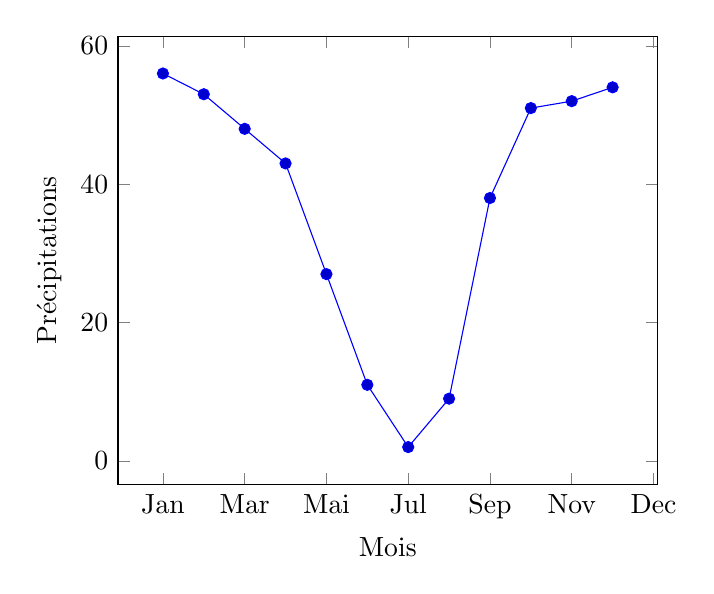
\begin{tikzpicture}
\begin{axis}[
ylabel=Précipitations,
xlabel=Mois,
symbolic x coords={Jan,Fev,Mar,Avr,Mai,Jun,Jul,Agu,
Sep,Oct,Nov,Dec},
%x tick label style={rotate=45,anchor=east}
%xtick distance=1
]
\addplot coordinates {
(Jan,56) (Fev,53) (Mar,48) (Avr,43) (Mai,27) (Jun,11) (Jul,2) (Agu,9) (Sep,38) (Oct,51) (Nov,52) (Dec,54)
};
\end{axis}
\end{tikzpicture}
\end{center}
\end{Ex}


\end{pageCours} 




\begin{pageAD} 

\Sf{Savoir lire un diagramme cartésien }

\ExoCad{Représenter.}

 
\Sf{Savoir lire un diagramme cartésien }

\ExoCad{Représenter. Calculer.}

 


\end{pageAD}



%%%%%%%%%%%%%%%%%%%%%%%%%%%%%%%%%%%%%%%%%%%%%%%%%%%%%%%%%%%%%%%%%%%
%%%%  Niveau 1
%%%%%%%%%%%%%%%%%%%%%%%%%%%%%%%%%%%%%%%%%%%%%%%%%%%%%%%%%%%%%%%%%%%
\begin{pageParcoursu} 

\ExoCu{Chercher. Communiquer.}

 
 
\end{pageParcoursu}


%%%%%%%%%%%%%%%%%%%%%%%%%%%%%%%%%%%%%%%%%%%%%%%%%%%%%%%%%%%%%%%%%%%
%%%%  Niveau 2
%%%%%%%%%%%%%%%%%%%%%%%%%%%%%%%%%%%%%%%%%%%%%%%%%%%%%%%%%%%%%%%%%%%
\begin{pageParcoursd} 


\ExoCd{Représenter. Calculer.} 

 
 
 
 
\end{pageParcoursd}

%%%%%%%%%%%%%%%%%%%%%%%%%%%%%%%%%%%%%%%%%%%%%%%%%%%%%%%%%%%%%%%%%%%
%%%%  Niveau 3
%%%%%%%%%%%%%%%%%%%%%%%%%%%%%%%%%%%%%%%%%%%%%%%%%%%%%%%%%%%%%%%%%%%
\begin{pageParcourst}


\ExoCt{Modéliser. Calculer.}

 
 
\end{pageParcourst}

%%%%%%%%%%%%%%%%%%%%%%%%%%%%%%%%%%%%%%%%%%%%%%%%%%%%%%%%%%%%%%%%%%%
%%%%  Brouillon
%%%%%%%%%%%%%%%%%%%%%%%%%%%%%%%%%%%%%%%%%%%%%%%%%%%%%%%%%%%%%%%%%%%


\begin{pageBrouillon} 
 
\ligne{32}



\end{pageBrouillon}



\begin{pageAuto} 

\ExoAuto
 
\ExoAuto
 



\ExoAuto

 

 



\end{pageAuto}



